\documentclass[a4paper, 12pt]{article}
\usepackage[a4paper,top=1.5cm, bottom=1.5cm, left=1cm, right=1cm]{geometry}
\usepackage{cmap}					% поиск в PDF
\usepackage{mathtext} 				% русские буквы в формулах
\usepackage[T2A]{fontenc}			% кодировка
\usepackage[utf8]{inputenc}			% кодировка исходного текста
\usepackage[english,russian]{babel}	% локализация и переносы

\usepackage{amsmath,amssymb}
\usepackage{indentfirst}
\usepackage{longtable}
\usepackage{graphicx}
\usepackage{array}
\usepackage{float}

\usepackage{floatflt}
\usepackage{wrapfig}
\usepackage{siunitx} % Required for alignment
\usepackage{subfigure}
\usepackage{multirow}
\usepackage{rotating}
\usepackage{caption}

\graphicspath{{.}}


\title{\begin{center}Лабораторная работа №5.10.1\end{center}
Электронный парамагнитный резонанс}
\author{Рожков А. В.}
\date{\today}

\begin{document}
    \pagenumbering{gobble}
    \maketitle
    \newpage
    \pagenumbering{arabic}
    \renewcommand*{\thesubsection}{\thesection.\Alph{subsection}}

    \textbf{Цель работы:} исследовать электронный парамагнитный резонанс в молекуле
ДФПГ, определяется $g$-фактор электрона, измерить ширину линии ЭПР.

    \section{Теоретическое введение}

        Энергетический уровень электрона в присутствии магнитного поля с индукцией $B$ расщепляется на подуровня, расстояние между которыми равно
        \begin{equation}
            \label{eq:dE}
            \Delta E = E_2 - E_1 = 2\mu B.
        \end{equation}
        Здесь $\mu$ -- абсолютная величина проекции магнитного момента на направление поля.

        Между этими двумя уровнями возможны переходы. Эти переходы могут возбуждаться внешним выскочастотным электромагнитным полем, если оно имеет нужную частоту и нужное направление.

        Резонансное значение частоты определяется из очевидной формулы:
        \begin{equation}
            \label{eq:resonans_omega}
            \hbar \omega_0 = \Delta E.
        \end{equation}

        При переходе с нижнего на верхний уровень энергии электрон поглощает квант электромагнитной энергии, а при обратном переходе такой же квант излучается.
        Возбуждение электронных резонансных переходов электромагнитным полем, имеющим частоту, определяемую формулой (\ref{eq:resonans_omega}),
        носит название \textit{электронного парамагнитного резонанса (ЭПР)}.

        Как известно, связь между магнитным моментом $\upmu$ электрона и его механическим моментом $\mathbf{M}$ выражается через гиромагнитное отношение $\gamma$ с помощью формулы
        \begin{equation}
            \label{eq:gyromagnit}
            \upmu = \gamma \mathbf{M}.
        \end{equation}

        Используя соотношения (\ref{eq:dE})-(\ref{eq:gyromagnit}), нетрудно получить выражение для $g$-фактора через определяемые экспериментально величины:
        \begin{equation}
            \label{eq:g-faktor}
            \tag{$\star$}
            g = \frac{\hbar \omega_0}{\mu_\text{Б}B}.
        \end{equation}

        Уширение линии поглощения происходит в основном за счёт спин-спинового взаимодействия
        (взаимодействие между магнитным моментом рассматриваемого электрона и магнитными моментами других электронов)
        и спин-решеточного взаимодействия (взаимодествие электрона с атомами и молекулами вещества).
        Спин-решеточное взаимодействие быстро возрастает с температурой (числом фононов),
        спин-спиновое взаимодействие от температуры практически не зависит.

    \section{Экспериментальная установка}

        Образец (порошок ДФПГ) в стеклянной ампуле помещяется внутрь катушки индуктивности входящей в состав колебательного контура.
        Входящий в состав контура конденсатор состоит из двух пластин, разделенных воздушным зазором, одна из пластин может перемещаться поворотом штока.
        Колебания в контуре возбуждаются антенной, соединённой с генератором частоты (ВЧ) Г4-116.
        Амплитуда колебаний поля в катушке индуктивности измеряется по наводимой в петле связи ЭДС индукции.
        Высокочастотные колебания ЭДС индукции в приёмном контуре детектируются диодом,
        измеряемая при помощи осциллографа низкочастотная огибающая этого сигнала пропорциональна квадрату амплитуды колебаний поля в катушке.


        Постоянное магнитное поле создаётся пропусканием тока от источника постоянного тока через основные катушки.
        При этом при помощи вольтметра измеряется падение напряжения на резисторе в цепи основных катушек.
        Переменное поле небольшой амплитуды создаётся подачей на модуляционные катушки напряжения с регулируемого трансформатора ЛАТР.
        Для измерения амплитуды колебаний переменного поля используется пробная катушка известной геометрии, подключенная к вольтметру.

        \begin{figure}[H]
            \centering
            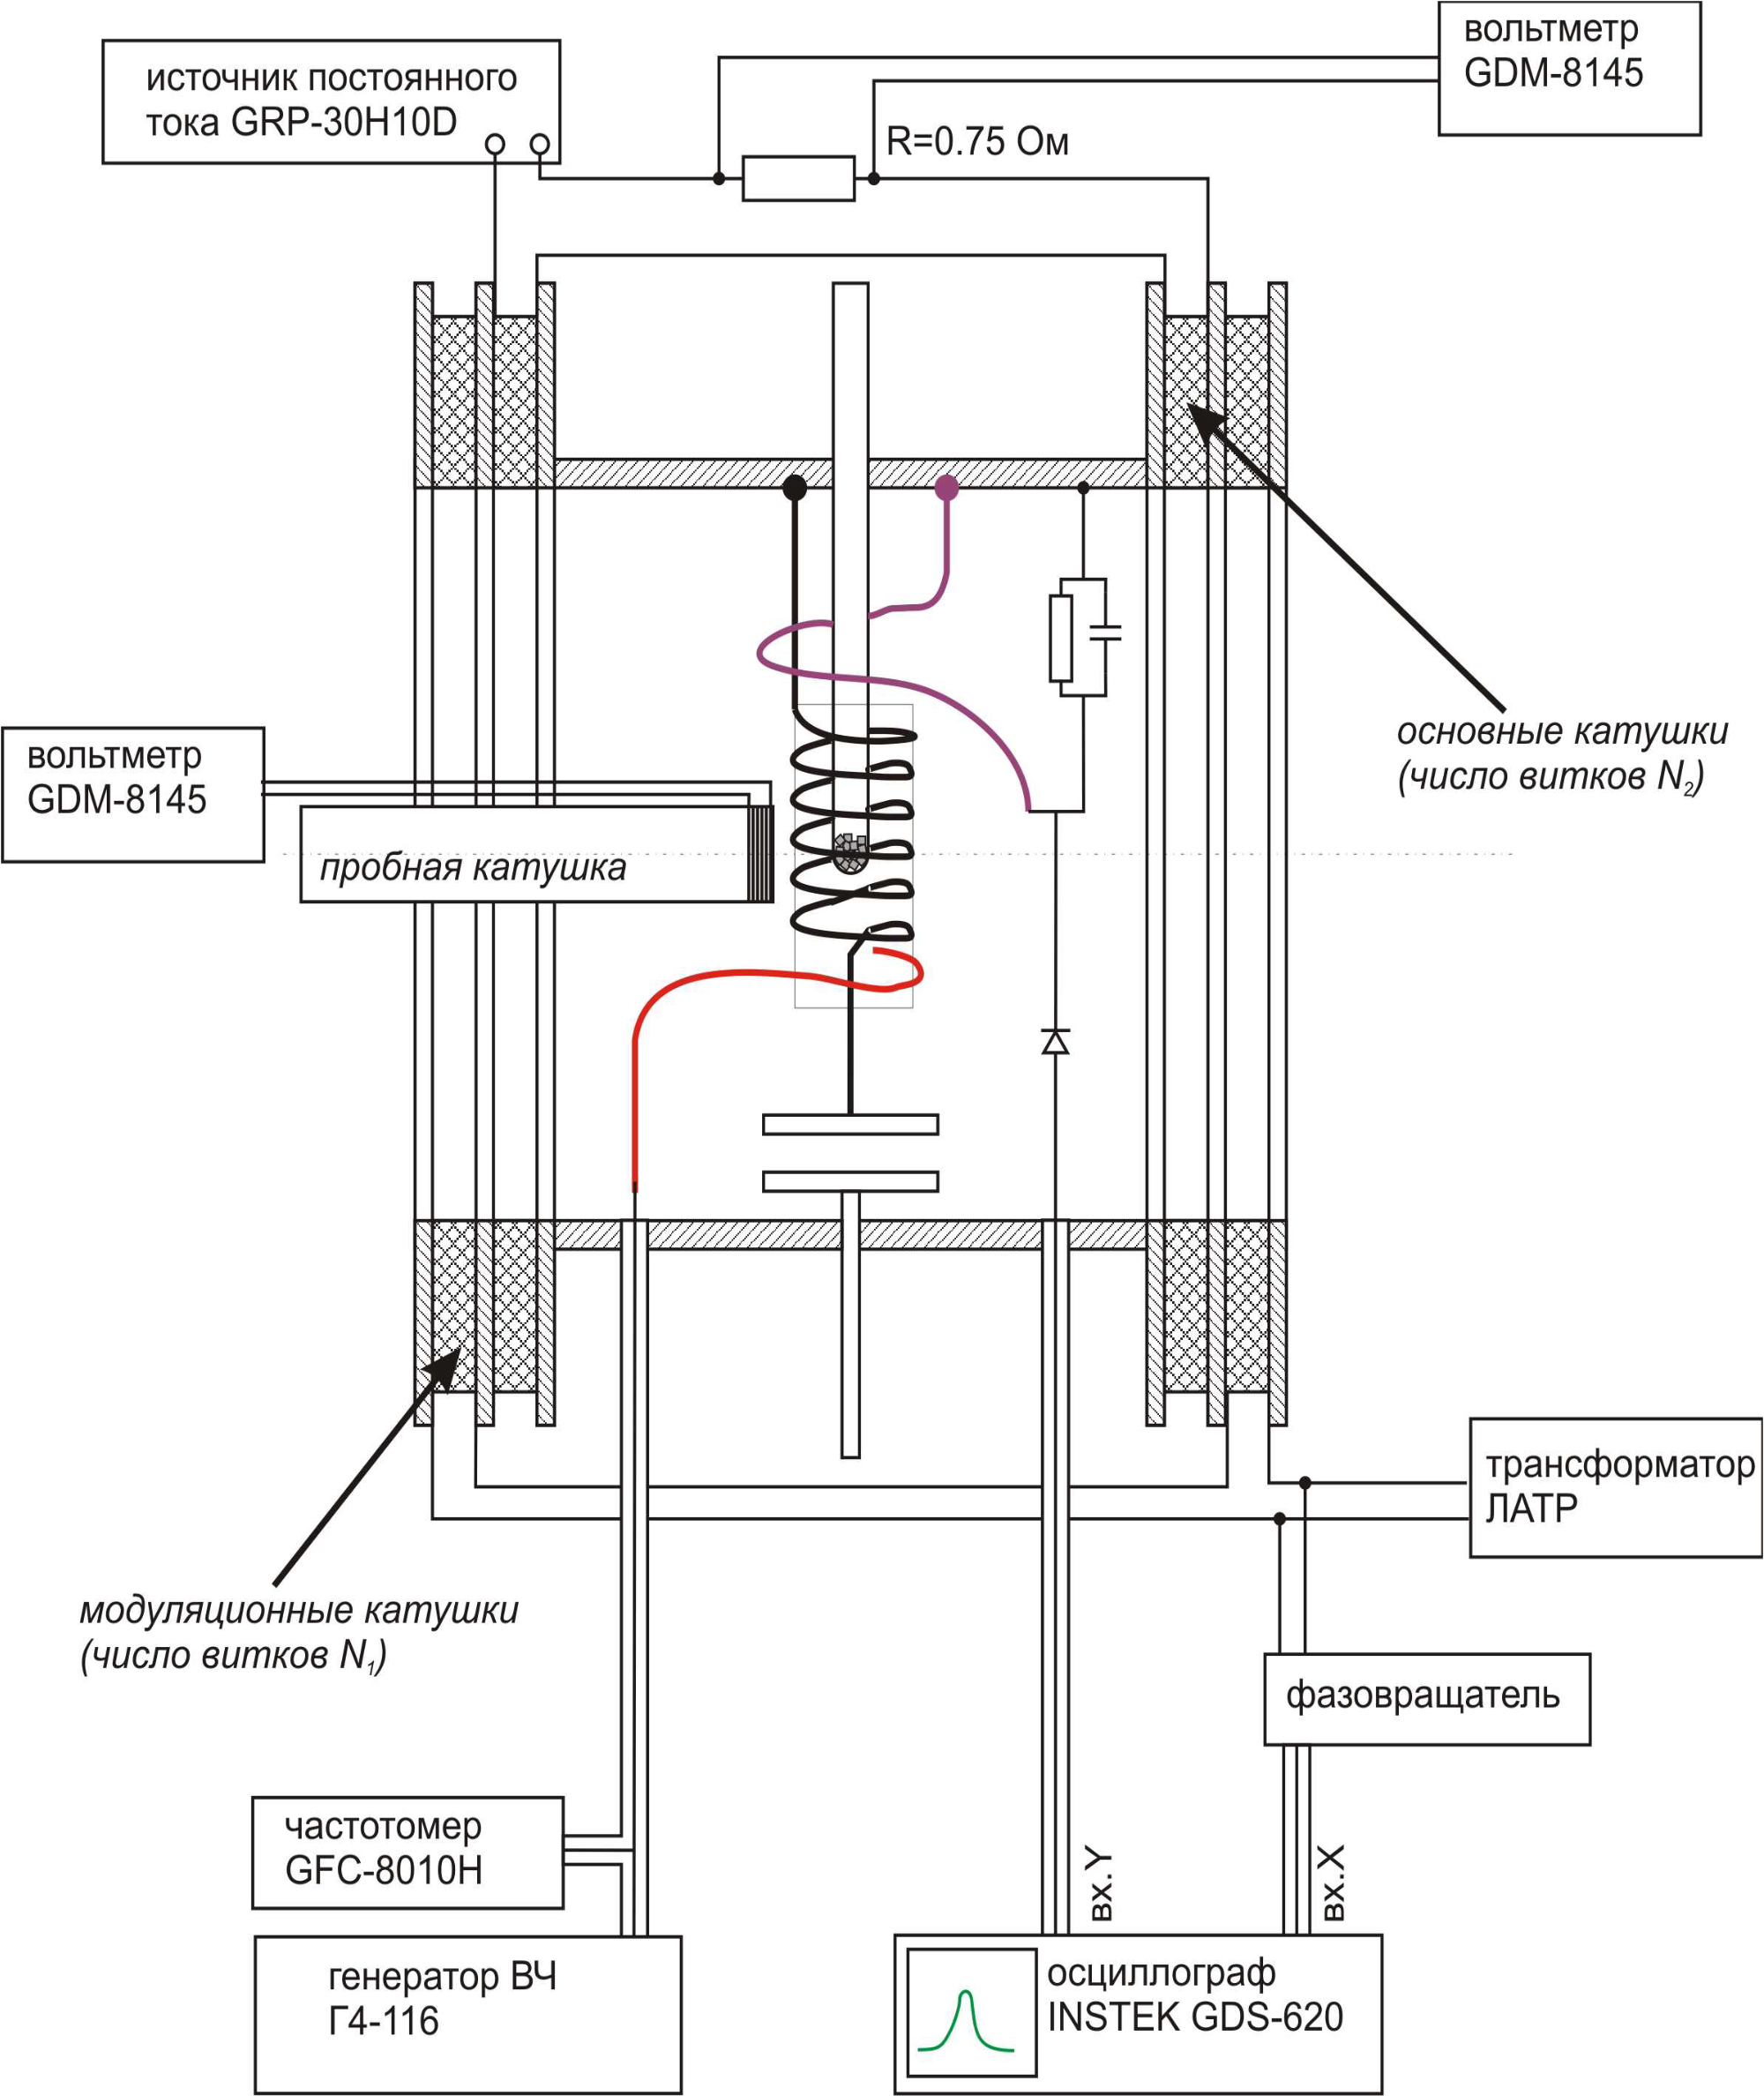
\includegraphics[width = 0.75\linewidth]{img/setup.png}
            \caption{Схема экспериментальной установки}
            \label{}
        \end{figure}


        \newpage
    \section{Ход работы}

        Настроим ВЧ генератор на частоту колебательного контура. В режиме непрерывной генерации ВЧ генератор выдаёт переменный (частота  $\sim  100$ МГц) сигнал постоянной амплитуды, который после детектирования превращается в постоянное напряжение. Наблюдение постоянного напряжения на экране осциллографа неудобно, поэтому для удобства настройки сигнал дополнительно амплитудно модулируется на низкой ( $\sim  1$ кГц) частоте.

        Детектирование усредняет высокочастотный сигнал, а его огибающая превращается в низкочастотный переменный сигнал, легко визуализуемый на осциллографе.

        \[ f_{\text{рез}} = (162.1 \pm 0.1) \text{ МГц} \]

        Подключим основные катушки к источнику постоянного тока, а модуляционные катушки к трансформатору ЛАТР. Подадим на модуляционные катушки напряжение  $\sim 50$ В (по вольтметру на ЛАТР).

        Увеличивая постоянное напряжение, подаваемое на основные катушки, добьёмся возникновения на экране осциллографа картины резонансного поглощения.

        Подадим на X-канал осциллографа напряжение, прикладываемое к модуляционным катушкам и будем наблюдать сигнал в XY-режиме.

        При точной настройке постоянного поля наблюдаемая картина должна быть симметрична относительно средней вертикальной оси.

        Совмещаем пики с помощью фазовращателя и подстроим немного частоту, добиваясь возникновения симметричного сигнала максимальной амплитуды.

        Запишем напряжение на резисторе в цепи основных катушек и подстроенную частоту:
        \[ U_0 = (179 \pm 1) \text{ мВ} \]
        \[ f_0 = (162.1 \pm 0.1) \text{ MГц} \]

        Для определения поля резонансного поглощения необходимо найти связь между падением напряжения на резисторе в цепи основной катушки и магнитным полем.
        Это можно сделать, если подать в основные катушки переменный ток и измерить при помощи пробной катушки ЭДС индукции. Подключим основные катушки на ЛАТР.

        \begin{table}[!ht]
            \centering
            \begin{tabular}{|c|c|c|}
                \hline

                $U_r, мВ$ & $\epsilon_{спереди}, мВ$ & $\epsilon_{сзади}, мВ$\\ \hline
                10.1 & 0.09 & 0.07\\ \hline
                29.8 & 2.59 & 2.05\\ \hline
                70.0 & 5.88 & 4.78\\ \hline
                120.3 & 10.13 & 8.27\\ \hline
                160.5 & 13.42 & 10.91\\ \hline
                180.1 & 15.03 & 12.28\\ \hline
                199.2 & 16.61 & 13.53\\ \hline

            \end{tabular}
            \caption{Результаты измерений при помощи пробной катушки}
            \label{}
        \end{table}

        Построим график зависимости ЭДС индукции в пробных катушках от напряжения на резисторе в цепи основных катушек.

        \begin{figure}[H]
            \centering
            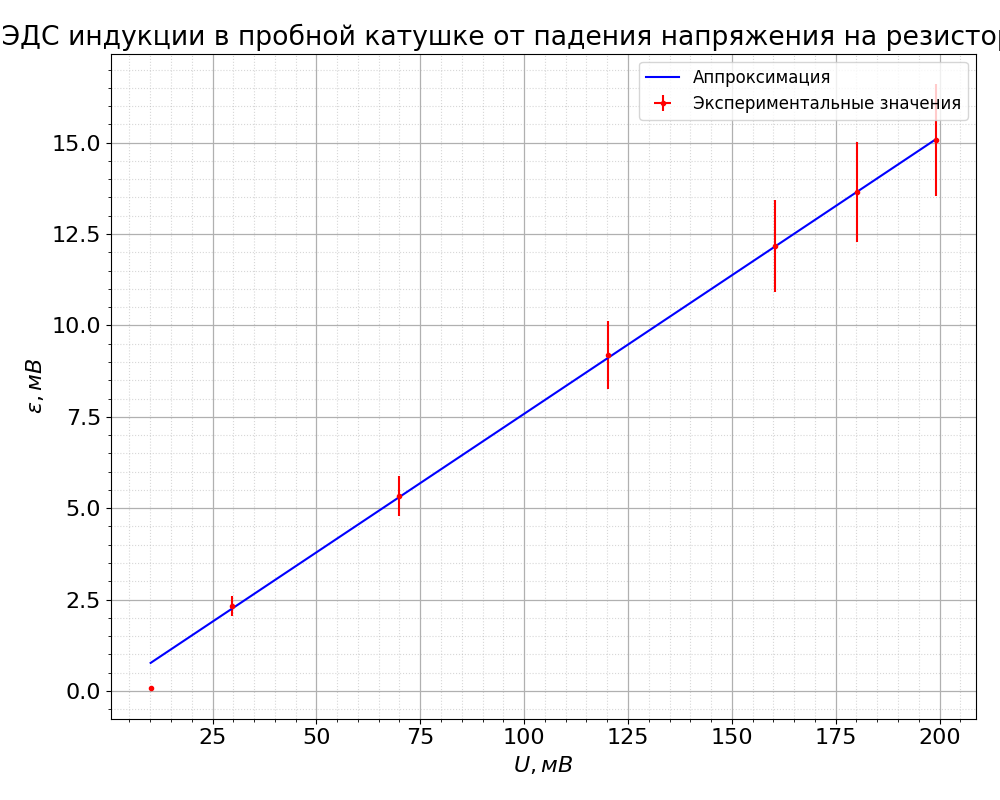
\includegraphics[width = 0.75\linewidth]{img/probe_plot.png}
            \caption{График зависимости ЭДС индукции в пробной катушке от напряжения на резисторе в цепи основных катушек}
            \label{}
        \end{figure}

        Проведём прямую по МНК. Коэффициент наклона прямой равен $k = (0.0758 \pm 0.0008)$.

        Для определения ширины линии ЭПР определим по экрану осциллографа полный размах модулирующего поля (в делениях шкалы) $A_{\text{полн}}$ и полную ширину кривой резонансного поглощения на полувысоте $A_{1/2}$.

        \[ A_{\text{полн}} = 6.8 \pm 0.2, ~A_{1/2} = 0.5 \pm 0.2 \]

        При этом определим ЭДС индукции, создающееся в центре катушки:

        \[ \varepsilon_{\text{инд}} = (4.4 \pm 0.1) \text{ мВ}\]

        Параметры пробной катушки: $N = 44$, $d = (14.5 \pm 0.1) \text{ мм}$, частота модулирующего напряжения $\nu = (50 \pm 5) \text{ Гц}$.

        \[B_{\text{мод}} =  \sqrt{2} \frac{2 \varesilon_{\text{инд}}}{\pi^2 d^2 N \nu} = (1.8 \pm 0.2) \text{ мТл}\]

        Полуширина на полувысоте линии резонансного поглощения может быть тогда получена как

        \[ \Delta B = \frac{A_{1/2}}{A_{\text{полн}}}B_{\text{мод}} = (0.13 \pm 0.06) \text{ мТл} \]

        Посчитаем индукцию постоянного магнитного поля
        \[ B_0 = \frac{2 \varepsilon_{инд}(U_0)}{\pi^2 d^2 N \nu} = (5.6 \pm 0.6) \text{ мТл}\]

        где $\varepsilon_{\text{инд}}(U_0) = (13.6 \pm 0.6) \text{ мВ}$

        Формула для $g$-фактора имеет следующий вид:
        \[ g = \frac{h f_0}{\mu_B B_0} = 2.1 \pm 0.2\]

    \section{Заключение}

        В данной работе был исследован ЭПР в молекуле ДФПГ, определяется $g$-фактор электрона $g = 2.1 \pm 0.2$, а также измерена ширина линий ЭПР $\Delta B = (0.13 \pm 0.06) ~ \text{мТл}$.

\end{document}
